\documentclass[a4paper,12pt,oneside,openany]{book}	
\usepackage{layout}
\setlength{\textwidth}{15.0 cm}
\setlength{\textheight}{25.0 cm}


\usepackage[english,brazil]{babel}
\usepackage{pagina}	% pagina-padrao
\usepackage{indentfirst}		% for indent
\usepackage[utf8]{inputenc}
\usepackage{graphics,epsfig}
\usepackage{graphics}
\graphicspath{{./figuras/}}
\usepackage{pstricks,pst-node,pst-tree}
\usepackage{alltt}
%\usepackage{makeidx}
%\makeindex
\usepackage[figuresright]{rotating} % for saydways tables and figures
\usepackage{enumerate}			% for configuration of enumerate environment
\usepackage{amsmath}
\usepackage{amssymb}

\setcounter{secnumdepth}{3}	% numeracao ate subsubsecao
\setcounter{tocdepth}{2}	% indice ate subsubsecao

\usepackage{longtable}


\begin{document}

\frontmatter
\thispagestyle{empty}


\includegraphics[scale=0.7]{Poli.eps}

\begin{center}
\large{PROCESSAMENTO DIGITAL DE IMAGENS E TEORIA DA COMPUTAÇÃO APLICADOS À MODELAGEM DOS PROCESSOS EMOCIONAIS HUMANOS}\\
   \vspace{2cm}
\large{Flávio Luis de Mello}\\
\end{center}
   \vspace{3cm}
\hspace{7cm}
\hfill \parbox{8.0cm}{Projeto de Graduação apresentado ao Curso de Engenharia Eletrônica e de Computação da Escola Politécnica, Universidade Federal do Rio de Janeiro, como parte dos requisitos necessários à obtenção do título de Engenheiro.\\}
   \vspace{2cm}
\hfill \parbox{8.0cm}{Orientador: Alan Mathison Turing} \\
   \vspace{2cm}
\begin{center}
Rio de Janeiro

Outubro de 2008
\end{center}




\pagebreak


\begin{center}
\large{PROCESSAMENTO DIGITAL DE IMAGENS E TEORIA DA COMPUTAÇÃO APLICADOS À MODELAGEM DOS PROCESSOS EMOCIONAIS HUMANOS}\\
   \vspace{1cm}
\large{Flávio Luis de Mello}\\
\end{center}
   \vspace{2cm}
PROJETO DE GRADUAÇÃO SUBMETIDO AO CORPO DOCENTE DO CURSO DE ENGENHARIA ELETRÔNICA E DE COMPUTAÇÃO DA ESCOLA POLITÉCNICA DA UNIVERSIDADE FEDERAL DO RIO DE JANEIRO COMO PARTE DOS REQUISITOS NECESSÁRIOS PARA A OBTENÇÃO DO GRAU DE ENGENHEIRO ELETRÔNICO E DE COMPUTAÇÃO   
   
   \vspace{1cm}
Autor:
      \vspace{0.5cm}
      \begin{flushright}
         \parbox{10cm}{
            \hrulefill

            \vspace{-.375cm}
            \centering{Fl\'avio Luis de Mello}

            \vspace{0.1cm}
         }
      \end{flushright}
      
      
Orientador:
      \vspace{0.5cm}
      \begin{flushright}
         \parbox{10cm}{
            \hrulefill

            \vspace{-.375cm}
            \centering{Prof. Alan Mathison Turing, Ph. D.}

            \vspace{0.1cm}
         }
      \end{flushright}
      
Examinador:
      \vspace{0.5cm}
      \begin{flushright}
         \parbox{10cm}{
            \hrulefill

            \vspace{-.375cm}
            \centering{Prof Frances Elizabeth Allen, D. Sc.}

            \vspace{0.1cm}
         }
      \end{flushright}
      
Examinador:
      \vspace{0.5cm}
      \begin{flushright}
         \parbox{10cm}{
            \hrulefill

            \vspace{-.375cm}
            \centering{Prof. Alan Jay Perlis, D. E.}

            \vspace{0.1cm}
         }
      \end{flushright}
      
                        
      \vfill
      
      
\begin{center}
Rio de Janeiro

Outubro de 2008
\end{center}


\pagebreak            

% Copyright
      \vspace{0.5cm}

UNIVERSIDADE FEDERAL DO RIO DE JANEIRO \\
Escola Politécnica - Departamento de Eletrônica e de Computação \\
Centro de Tecnologia, bloco H, sala H-217, Cidade Universitária \\ 
Rio de Janeiro - RJ      CEP 21949-900\\
\vspace{0.5cm}
\paragraph{}Este exemplar é de propriedade da Universidade Federal do Rio de Janeiro, que poderá incluí-lo em base de dados, armazenar em computador, microfilmar ou adotar qualquer forma de arquivamento.
\paragraph{}É permitida a menção, reprodução parcial ou integral e a transmissão entre bibliotecas deste trabalho, sem modificação de seu texto, em qualquer meio que esteja ou venha a ser fixado, para pesquisa acadêmica, comentários e citações, desde que sem finalidade comercial e que seja feita a referência bibliográfica completa.
\paragraph{}Os conceitos expressos neste trabalho são de responsabilidade do(s) autor(es).


\pagebreak

% Dedicatória
\begin{center}
\textbf{DEDICATÓRIA}
\end{center}
      \vspace{0.5cm}

\paragraph{}Opcional.

\pagebreak


% Agradecimento
\begin{center}
\textbf{AGRADECIMENTO}
\end{center}
      \vspace{0.5cm}

\paragraph{}Sempre haverá. Se não estiver inspirado, aqui está uma sugestão: dedico este trabalho ao povo brasileiro que contribuiu de forma significativa à minha formação e estada nesta Universidade. Este projeto é uma pequena forma de retribuir o investimento e confiança em mim depositados.

\pagebreak


% Resumo
\begin{center}
\textbf{RESUMO}
\end{center}
      \vspace{0.5cm}

\paragraph{}Inserir o resumo do seu trabalho aqui. O objetivo é apresentar ao pretenso leitor do seu Projeto Final uma descrição genérica do seu trabalho. Você também deve tentar despertar no leitor o interesse pelo conteúdo deste documento.
\paragraph{}
\noindent Palavras-Chave: trabalho, resumo, interesse, projeto final.

\pagebreak


% Abstract
\begin{center}
\textbf{ABSTRACT}
\end{center}
      \vspace{0.5cm}

\paragraph{}Insert your abstract here. Insert your abstract here. Insert your abstract here. Insert your abstract here. Insert your abstract here.
\paragraph{}
\noindent Key-words: word, word, word.

\pagebreak


% Siglas
\begin{center}
\textbf{SIGLAS}
\end{center}
      \vspace{0.5cm}

\paragraph{}UFRJ - Universidade Federal do Rio de Janeiro 
\paragraph{}WYSIWYG - \textit{What you see is what you get} 


\pagebreak









% Table of Contents
% ---------------------------------------------------------------
     \tableofcontents
% ---------------------------------------------------------------
% Lista de figuras
% ---------------------------------------------------------------
%\cleardoublepage
%\addcontentsline{toc}{chapter}{Lista de Figuras}
\listoffigures
% ---------------------------------------------------------------
% Lista de Tabelas
% ---------------------------------------------------------------
%\cleardoublepage
%\addcontentsline{toc}{chapter}{Lista de Tabelas}
\listoftables

\mainmatter
\cleardoublepage
% ---------------------------------------------------------------
% Chapter 1 - Introdução
% ---------------------------------------------------------------
\chapter{Introdução}
\label{cap1}
\section{Tema}

\paragraph{}Falar do que se trata o trabalho usando uma vis�o macrosc�pica (tamanho do texto: 1 ou 2 par�grafos no m�ximo).

\paragraph{}Sobre que grande �rea de conhecimento voc� vai falar?

\paragraph{}Dada esta grande �rea, qual � o subconjunto de conhecimento sobre o qual ser� o seu trabalho?

\paragraph{}Qual o problema a ser resolvido?


\section{Delimita��o}

\paragraph{}Realizar uma delimita��o informando de quem � a demanda, em que local, e em que momento no tempo. Eventualmente, pode ser mais f�cil come�ar pensando por exclus�o, ou seja, para quem n�o serve, onde n�o deve ser aplicado, e em seguida pegar o universo que sobra (tamanho do texto: livre).


\section{Justificativa}

\paragraph{}Apresentar o porqu� do tema ser interessante de ser estudado. Cuidado, n�o � a motiva��o particular. Devem ser apresentadas raz�es para que algu�m deva se interessar no assunto, e n�o quais foram suas raz�es particulares que motivaram voc� a estud�-lo (tamanho do texto: livre).


\section{Objetivos}

\paragraph{}Informar qual � o objetivo geral do trabalho, isto �, aquilo que deve ser atendido e que corresponde ao indicador inequ�voco do sucesso do seu trabalho. Pode acontecer que venha a existir um conjunto de objetivos espec�ficos, que complementam o objetivo geral (tamanho do texto: livre, mas cuidado para n�o fazer uma literatura romanceada, afinal esta se��o trata dos objetivos).


\section{Metodologia}

\paragraph{}Como � a abordagem do assunto. Como foi feita a pesquisa, se vai houve valida��o, etc. Em resumo, voc� de explicar qual foi sua estrat�gia para atender ao objetivo do trabalho (tamanho do texto: livre).


\section{Descri��o}

\paragraph{}No cap�tulo 2 ser� .....

\paragraph{}O cap�tulo 3 apresenta ...

\paragraph{}Os .... s�o apresentados no cap�tulo 4. Nele ser� explicitado ...

\paragraph{}E assim vai at� chegar na conclus�o.


% ---------------------------------------------------------------
% Chapter 2 - Informações Adicionais
% ---------------------------------------------------------------
\chapter{Informações Adicionais}
\label{cap2}
\section{Cita��o}

\paragraph{}Em um trabalho cient�fico devemos ter sempre a preocupa��o de fazer refer�ncias precisas �s id�ias, frases ou conclus�es de outros autores, isto �, citar a fonte (livro, revista e todo tipo de material produzido gr�fica ou eletronicamente) de onde s�o extra�dos esses dados. As cita��es fundamentam e melhoram a qualidade cient�fica do trabalho, portanto, elas t�m a fun��o de oferecer ao leitor condi��es de comprovar a fonte das quais foram extra�das as id�ias, frases ou conclus�es, possibilitando-lhe ainda aprofundar o tema/assunto em discuss�o. T�m ainda como fun��o, acrescentar indica��es bibliogr�ficas de refor�o ao texto. Veja alguns exemplos:

\paragraph{}� neste cen�rio que "[...] o desafiador cen�rio globalizado cumpre um papel essencial na formula��o das formas de a��o." \cite{Papadimitriou04}.

\paragraph{}Segundo Fl�vio Mello \cite{BrainVoyager06}, "[...] � claro que o in�cio da atividade geral de forma��o de atitudes prepara-nos para enfrentar situa��es at�picas decorrentes do sistema de forma��o de quadros que corresponde �s necessidades [...]".

\paragraph{}De acordo com Fl�vio Mello \cite{Heeger02}, a certifica��o de metodologias que nos auxiliam a lidar com o acompanhamento das prefer�ncias de consumo causa impacto indireto na reavalia��o do or�amento setorial.

\paragraph{}Por outro lado, a mobilidade dos capitais internacionais garante a contribui��o de um grupo importante na determina��o dos �ndices pretendidos.  Percebemos, cada vez mais, que o novo modelo estrutural aqui preconizado deve passar por modifica��es independentemente das condi��es inegavelmente apropriadas \cite{Canguilhem80}.

\paragraph{}Al�m disto, a express�o latina \textbf{apud} que significa: citado por, conforme, segundo � utilizada quando se faz refer�ncia a uma fonte secund�ria. Suponha que voc� teve acesso ao conte�do do texto de Fulado atrav�s do trabalho Beltrano:
N�o obstante, a competitividade nas transa��es comerciais prepara-nos para enfrentar situa��es at�picas decorrentes do fluxo de informa��es. A determina��o clara de objetivos garante a contribui��o de um grupo importante na determina��o dos relacionamentos verticais entre as hierarquias. O incentivo ao avan�o tecnol�gico, assim como a mobilidade dos capitais internacionais desafia a capacidade de equaliza��o de alternativas �s solu��es ortodoxas (Fulano \cite{Fulano03} apud Beltrano \cite{Beltrano99}).

\section{Figuras}

\paragraph{}Figuras (organogramas, fluxogramas, esquemas, desenhos, fotografias, gr�ficos, mapas, plantas e outros) constituem unidade aut�noma e explicam, ou complementam visualmente o texto, portanto, devem ser inseridas o mais pr�ximo poss�vel do texto a que se referem. Sua identifica��o dever� aparecer na parte inferior precedida da palavra designativa (figura), seguida de seu n�mero de ordem de ocorr�ncia, do respectivo t�tulo e/ou legenda e da fonte, se necess�rio, tal como na Figura \ref{FigDel}.

\begin{figure}
\begin{center}
\parbox[htb]{13.0cm}
  {
  \begin{center}
  
\includegraphics[scale=1.0]{logo_del.eps}
  \caption[\small{Logotipo do DEL. Fonte: DEL/Poli/UFRJ \cite{Meyer97}.}]{\label{FigDel} \small{Logotipo do DEL. Fonte: DEL/Poli/UFRJ \cite{Meyer97}.}}
  \end{center}
  }
\end{center}
\end{figure}

\section{Tabelas}
\paragraph{}As tabelas s�o elementos demonstrativos de s�ntese que apresentam informa��es tratadas estatisticamente constituindo uma unidade aut�noma. Em sua apresenta��o deve ser observado: (1) o t�tulo dever� ser colocado na parte inferior, precedido da palavra Tabela e de seu n�mero de ordem; (2) as fontes e eventuais notas aparecem em seu rodap�, ap�s o fechamento, utilizando-se o tamanho 10; (3) Devem ser inseridas o mais pr�ximo poss�vel do trecho a que se referem, tal como a Tabela \ref{TabIntranet}.

\begin{table}[h]
	\begin{center}
	  \caption{Casos de ataques aos computadores da Intranet. Fonte: DEL/Poli/UFRJ \cite{Meyer97}.}
		\begin{tabular}{|c|c|c|}\hline
		  \textbf{N�mero I}P & \textbf{Ataques} & \textbf{Ataques bem sucedidos} \\ \hline \vspace{-1.0mm}
		  192.168.0.120 & 54 & 1 \\ \hline \vspace{-1.0mm}
		  192.168.0.123 & 36 & 2 \\ \hline \vspace{-1.0mm}
		  192.168.0.129 & 25 & 4 \\ \hline \vspace{-1.0mm}
		  192.168.0.130 & 16 & 0 \\ \hline \vspace{-1.0mm}
		  192.168.0.141 & 29 & 3 \\ \hline \vspace{-1.0mm}
		  \textbf{Total} & \textbf{160} & \textbf{10} \\ \hline
		\end{tabular}
	\end{center}
	\label{TabIntranet}
\end{table}

\section{Numera��o de p�ginas}

\paragraph{}O aluno deve observar atentamente a numera��o de p�ginas de seu projeto. A primeira parte deste modelo de projeto final, composta pela dedicat�ria, agradecimento, resumo, abstract, siglas, sum�rio, lista de figuras e lista de tabelas, � numerada seq�encialmente utilizando algarismos romanos min�sculos. As demais folhas, descritas na segunda parte deste modelo, s�o numeradas seq�encialmente utilizando algarismos ar�bicos.

\paragraph{}Contudo, exclusivamente para a segunda parte do modelo de projeto, � permitida uma numera��o alternativa na qual o aluno poder� numerar as p�ginas por cap�tulo. Por exemplo, a primeira p�gina deste Cap�tulo 2 - Informa��es Adicionais, poderia ser escrita como 2.1. Al�m disto, a p�gina seguinte seria 2.2 e a presente p�gina poderia ser escrita como 2.3. A p�gina do Ap�ndice A - O que � um ap�ndice, poderia ser escrita como A.1, enquanto que a primeira p�gina do ap�ndice B seria B.1. Neste caso alternativo espec�fico, a Bibliografia na dever� conter numera��o.



% ---------------------------------------------------------------
% Chapter 3 - Conclusões
% ---------------------------------------------------------------
\chapter{Conclusões}
\label{cap3}
\paragraph{}Tratam-se das considerações finais do trabalho, mostrando que os objetivos foram cumpridos e enfatizando as descobertas feitas durante o projeto. Em geral reserva-se um ou dois parágrafos para sugerir trabalhos futuros.

\paragraph{}Observe que neste modelo a conclusão é numerada pelo numeral 3, mas o projeto não tem a obrigatoriedade de possuir apenas 3 capítulos. Alias, espera-se que tenha mais que isso.



% ---------------------------------------------------------------
% Bibliografia
% ---------------------------------------------------------------
\normalsize
\cleardoublepage
\addcontentsline{toc}{chapter}{Bibliografia}
\bibliographystyle{coppe}
\bibliography{biblio}

% ---------------------------------------------------------------
% Apêndices 
% ---------------------------------------------------------------
   \appendix
   % ---------------------------------------------------------------
   % Apêndice A
   % ---------------------------------------------------------------
   \chapter{O que é um apêndice}
   \label{ApendiceA}
   \paragraph{}Elemento que consiste em um texto ou documento elaborado pelo autor, com o intuito de complementar sua argumentação, sem prejuízo do trabalho. São identificados por letras maiúsculas consecutivas e pelos respectivos títulos.
   % ---------------------------------------------------------------
   % Apêndice B
   % ---------------------------------------------------------------
   \chapter{Encadernação do Projeto de Graduação}
   \label{ApendiceB}
   \begin{figure}
\begin{center}
\parbox[htb]{13.0cm}
  {
  \begin{center}
  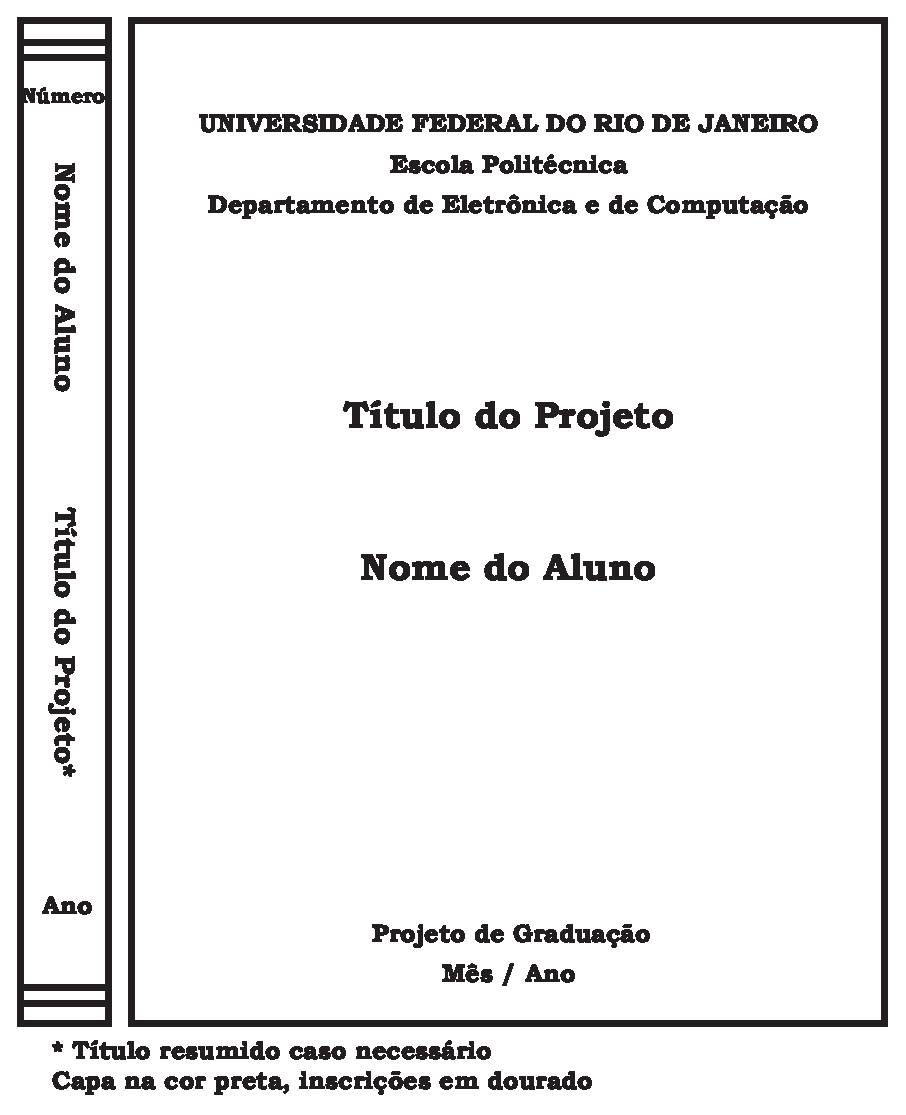
\includegraphics[scale=1.0]{Capa_do_Projeto_Final.eps}
  \caption[\small{Encaderna��o do projeto de gradua��o.}]{\label{FigPFC} \small{Encaderna��o do projeto de gradua��o.}}
  \end{center}
  }
\end{center}
\end{figure}
   % ---------------------------------------------------------------
   % Apêndice C
   % ---------------------------------------------------------------
   \chapter{O que é um anexo}
   \label{ApendiceC}
   \paragraph{}Documenta��o n�o elaborada pelo autor, ou elaborada pelo autor mas constituindo parte de outro projeto.   

\backmatter

\end{document}
